\section{Исследовательская часть}

В данном разделе будут приведены примеры работы программ и сравнительный анализ алгоритмов на основе полученных данных.

\subsection{Технические характеристики}

Технические характеристики устройства, на котором выполнялись замеры времени:
\begin{itemize}
    \item Процессор: \texttt{AMD Ryzen™ 7 4700U} 2.0 ГГц \cite{amd}, 8 физических ядер, 8 потоков;
    \item Оперативная память: 8 ГБ, \texttt{DDR4}, 3200 МГц;
    \item Операционная система: \texttt{NixOS 23.05.4448.5550a} \cite{nixos};
    \item Версия ядра: \texttt{6.1.59}.
\end{itemize}

\subsection{Демонстрация работы программы}

На рисунках \ref{fig:demo1} -- \ref{fig:demo3} представлена демонстрация работы программы: ручной ввод слов, проведение замеров времени и постровение графиков.

\begin{figure}[H]
	\centering
	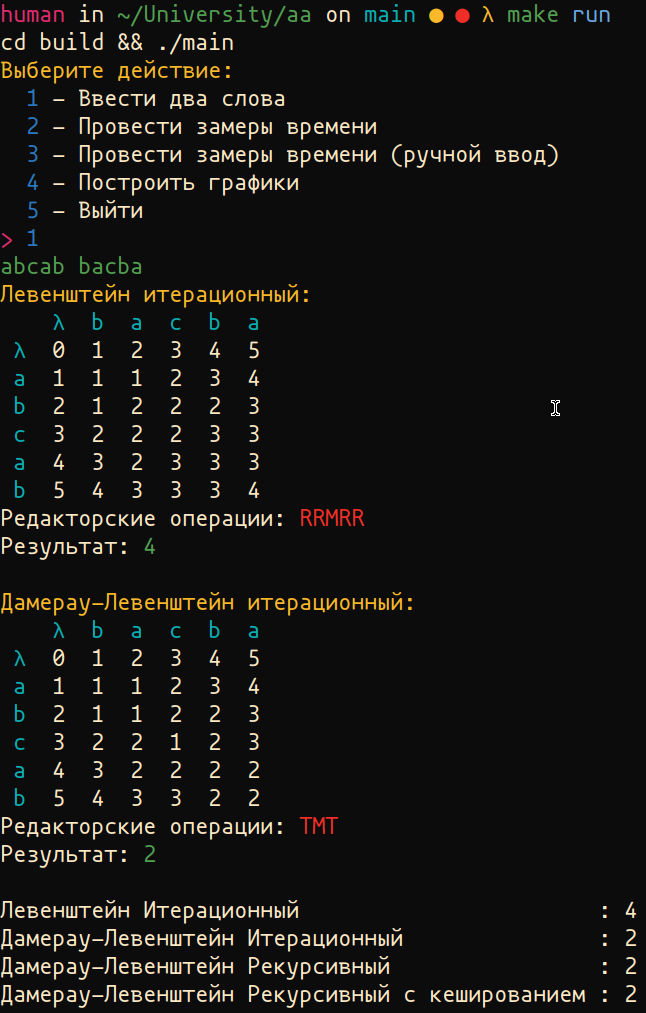
\includegraphics[scale=0.7]{img/demo1.png}
	\caption{Демонстрация работы программы, ввод двух слов}
	\label{fig:demo1}
\end{figure}

\begin{figure}[H]
	\centering
	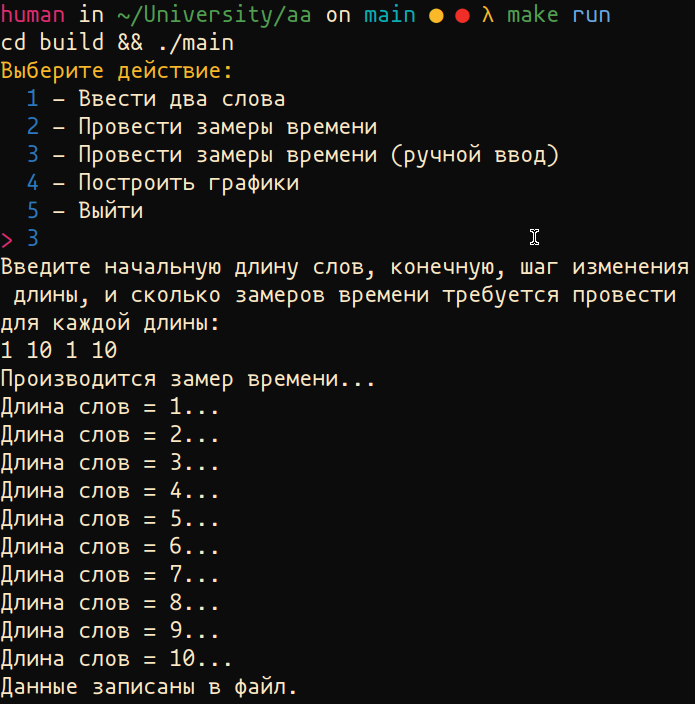
\includegraphics[scale=0.7]{img/demo2.png}
	\caption{Демонстрация работы программы, проведение замеров времени}
	\label{fig:demo2}
\end{figure}

\begin{figure}[H]
	\centering
	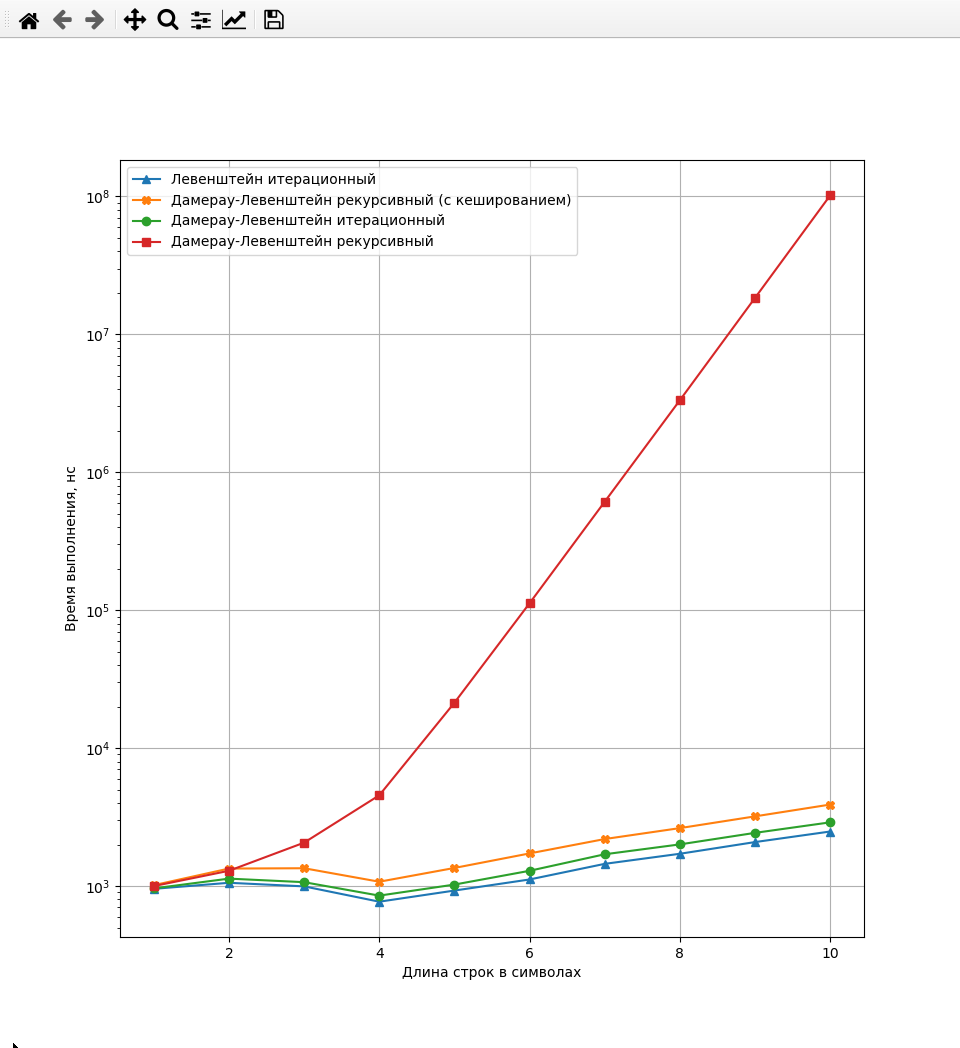
\includegraphics[scale=0.5]{img/demo3.png}
	\caption{Демонстрация работы программы, построение графиков на основе последних замеров времени (создаётся дочерний процесс, который запускает \texttt{Python}-скрипт)}
	\label{fig:demo3}
\end{figure}

\newpage

\subsection{Временные характеристики}

На графиках \ref{fig:fn_iter} -- \ref{fig:fn_four} представлены результаты замеров времени выполнения реализаций алгоритмов нахождения расстояний Левенштейна и Дамерау~---~Левенштейна.
Замеры времени проводились для строк одинаковой длины.
Отображённое на графиках время является усреднённым для каждой длины строк.

\begin{figure}[H]
	\centering
	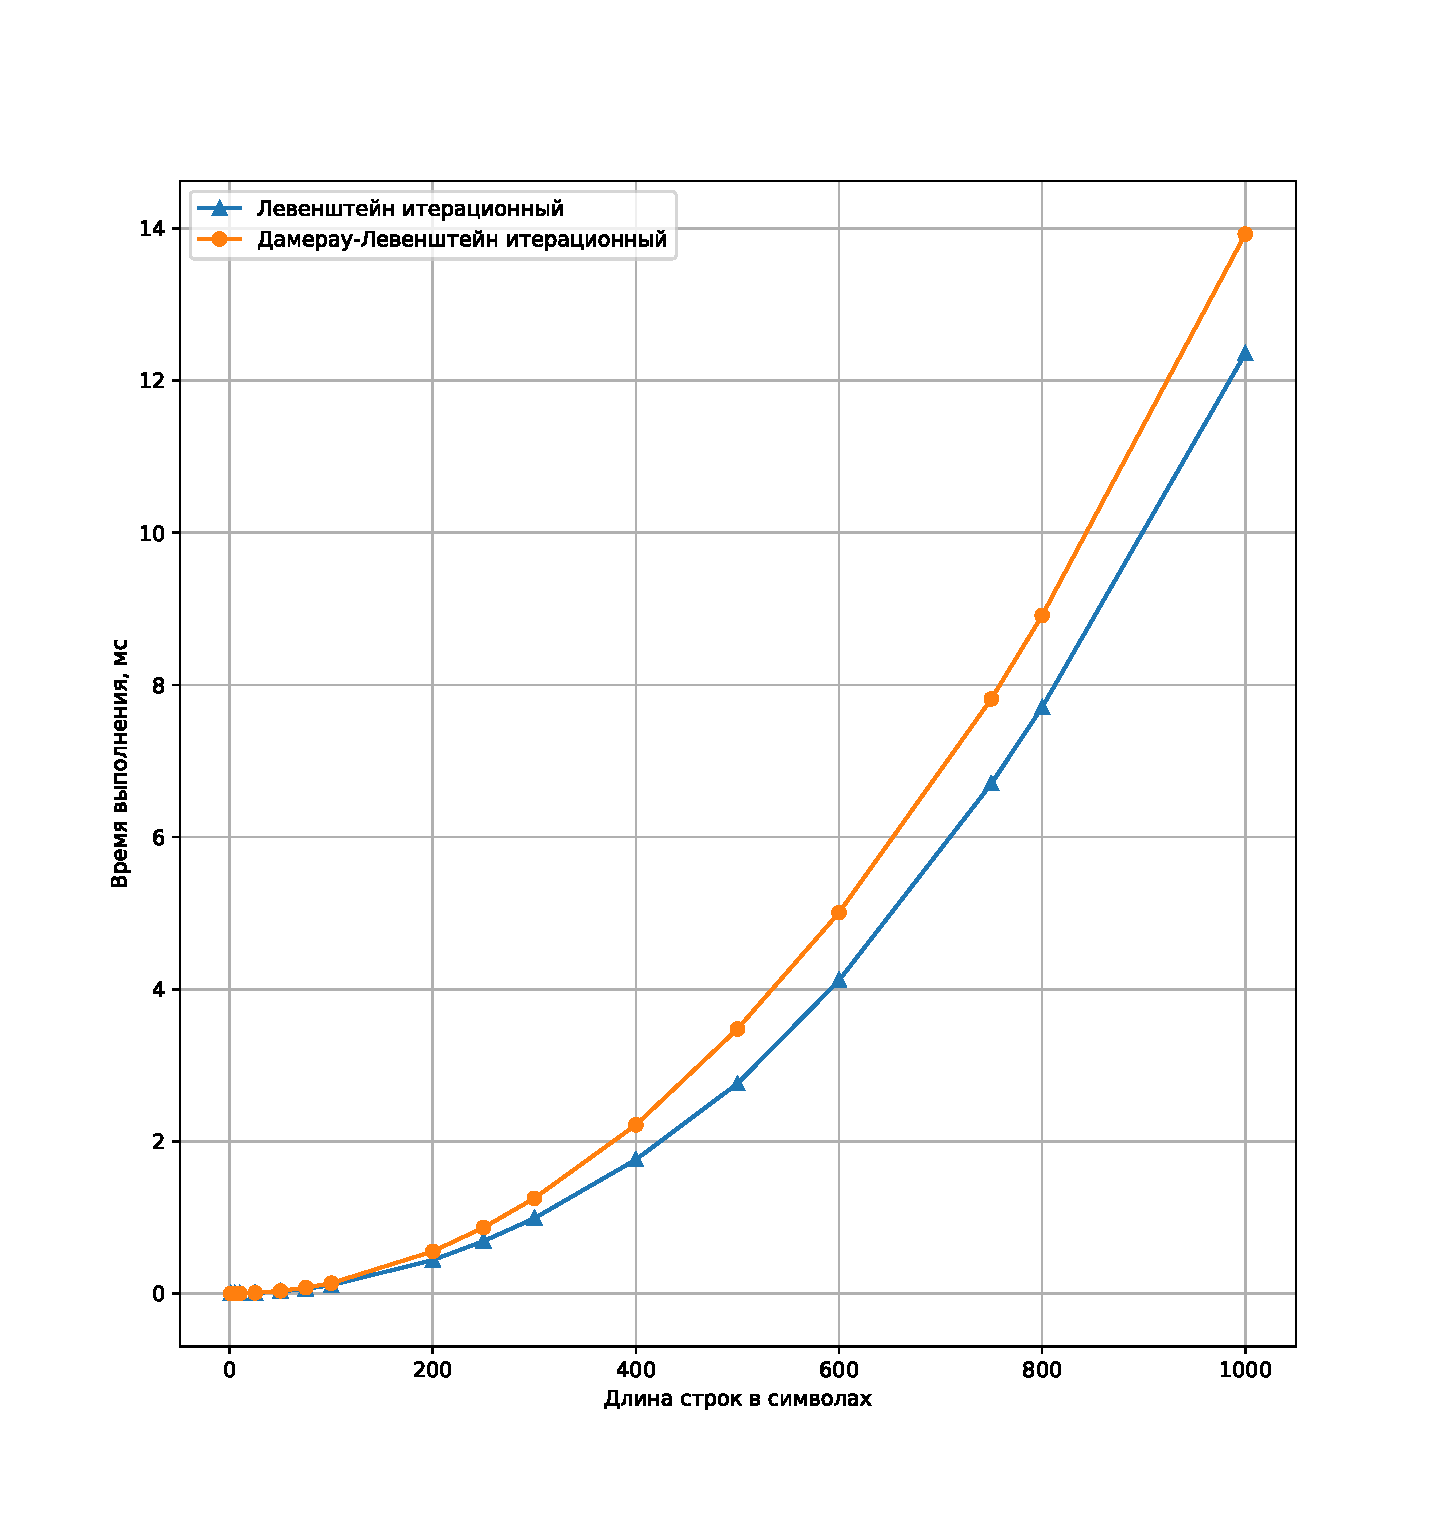
\includegraphics[width=\textwidth]{img/fn_iter.pdf}
	\caption{Сравнение реализаций итерационных алгоритмов по времени выполнения (среднее время из 100 замеров)}
	\label{fig:fn_iter}
\end{figure}

\begin{figure}[H]
	\centering
	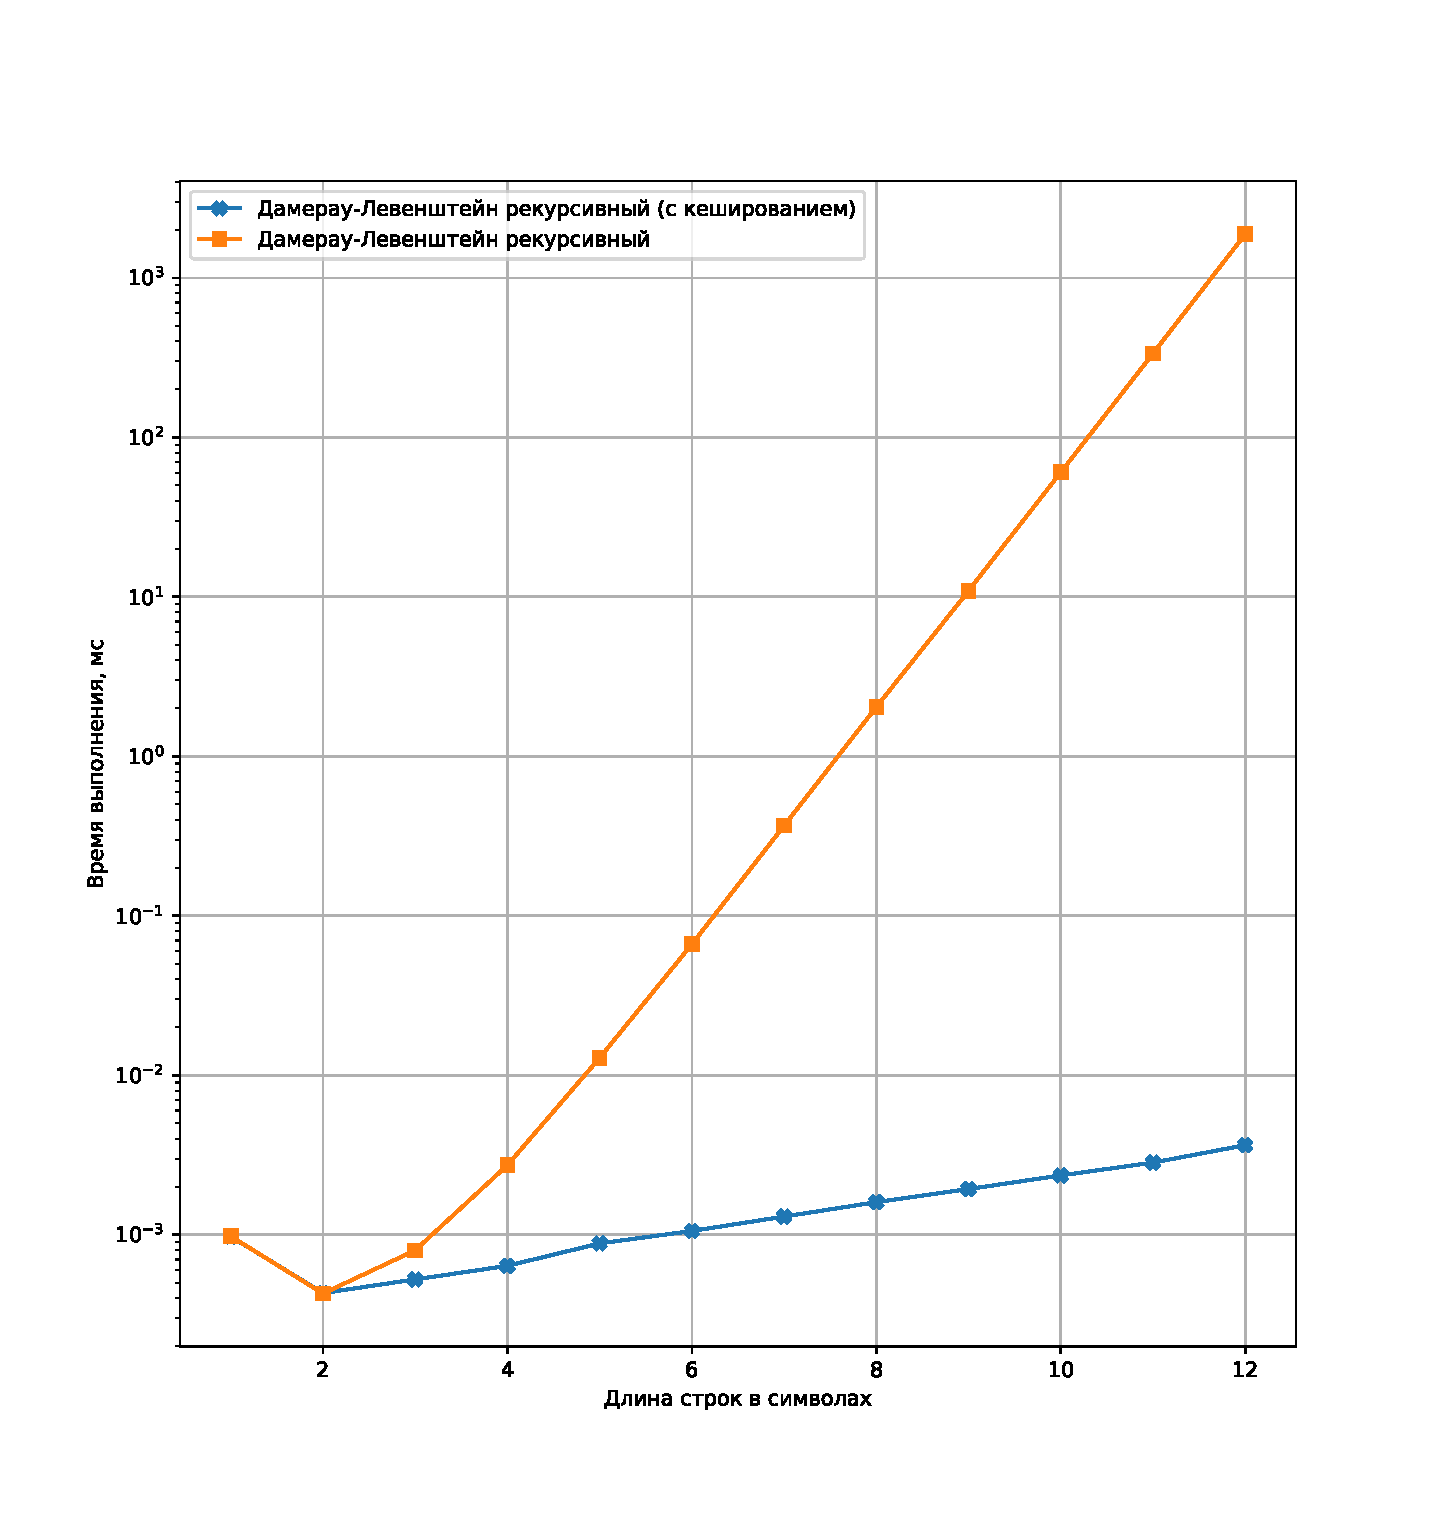
\includegraphics[width=\textwidth]{img/fn_rec.pdf}
	\caption{Сравнение реализаций рекурсивных алгоритмов по времени выполнения (среднее время из 10 замеров)}
	\label{fig:fn_rec}
\end{figure}

\begin{figure}[H]
	\centering
	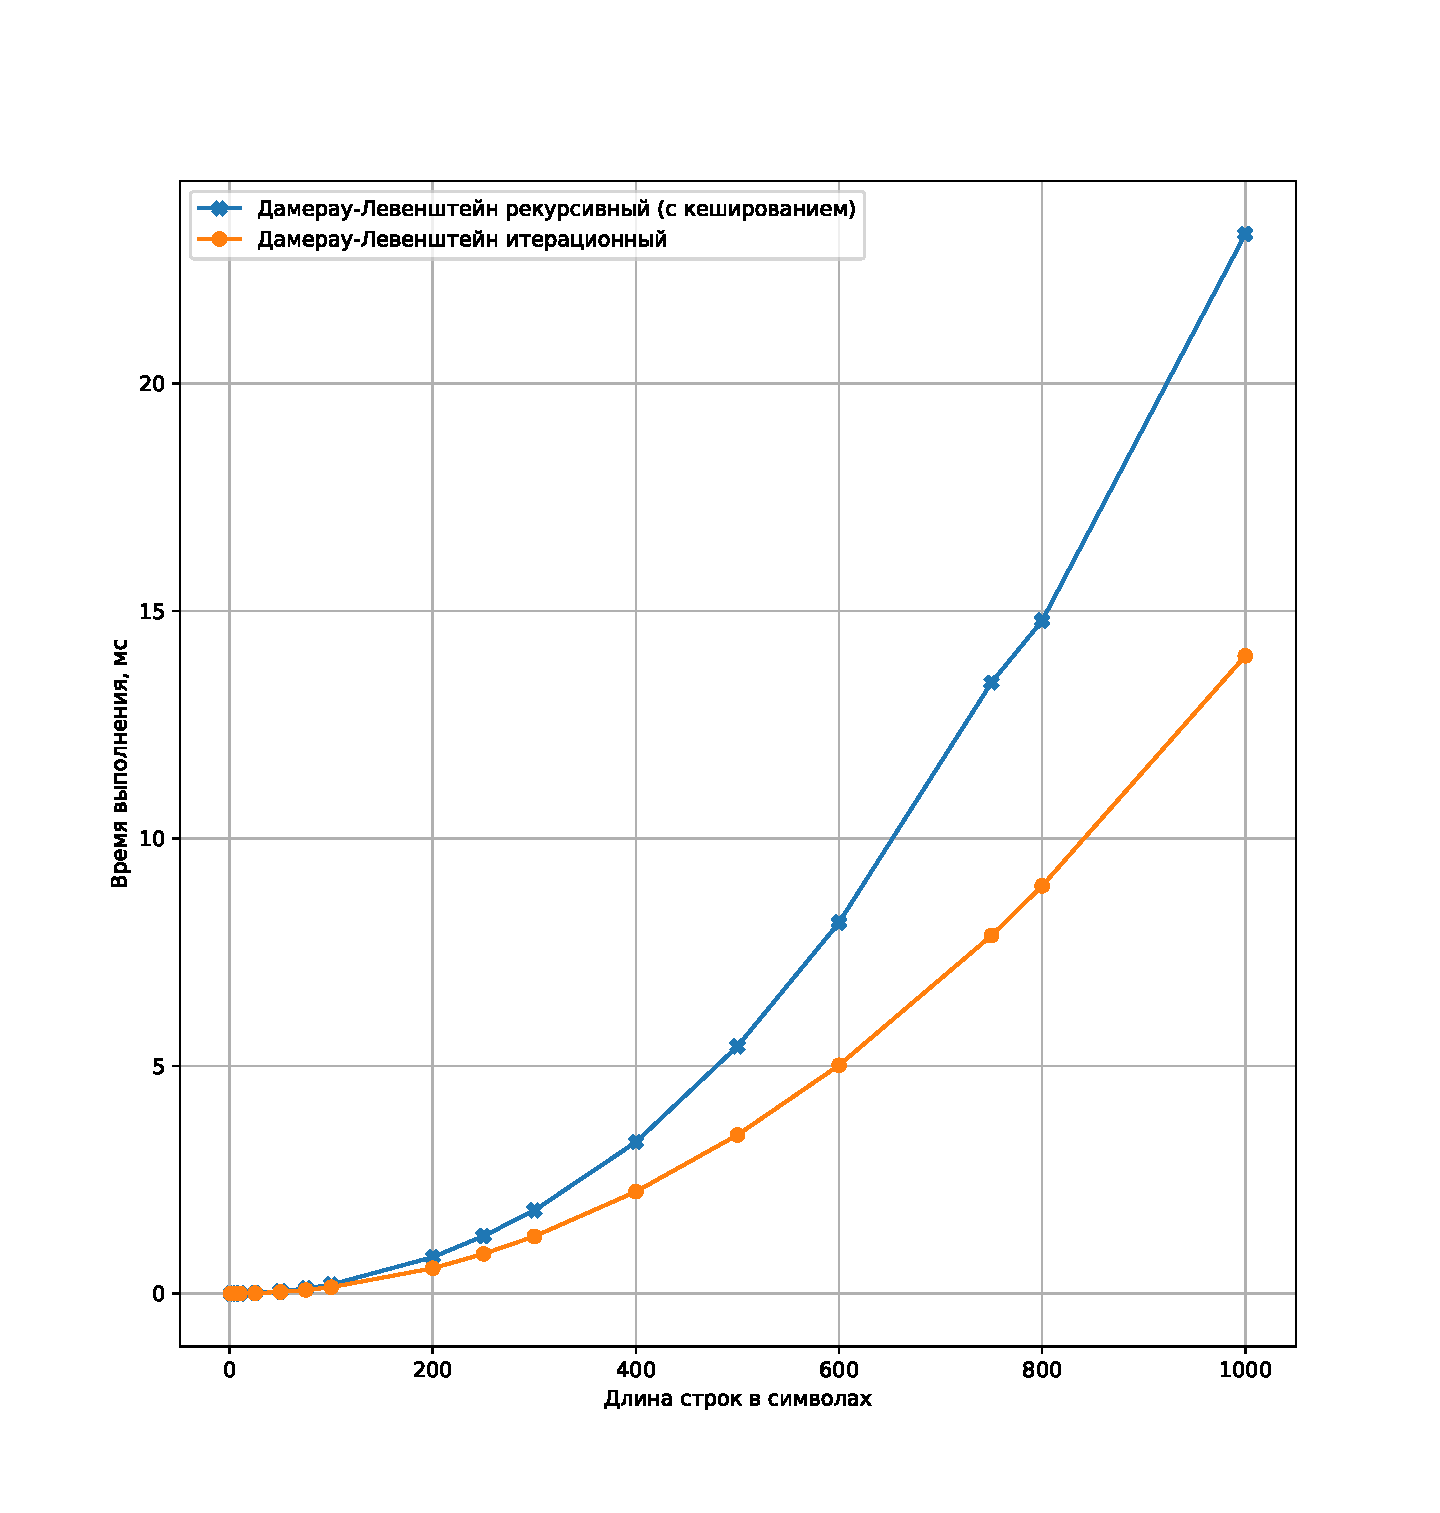
\includegraphics[width=\textwidth]{img/fn_damlev_iter_rec.pdf}
	\caption{Сравнение итерационной и рекурсивной с кешированием реализации алгоритмов нахождения расстояния Дамерау --- Левенштейна по времени выполнения (среднее время из 100 замеров)}
	\label{fig:fn_dlir}
\end{figure}

\begin{figure}[H]
	\centering
	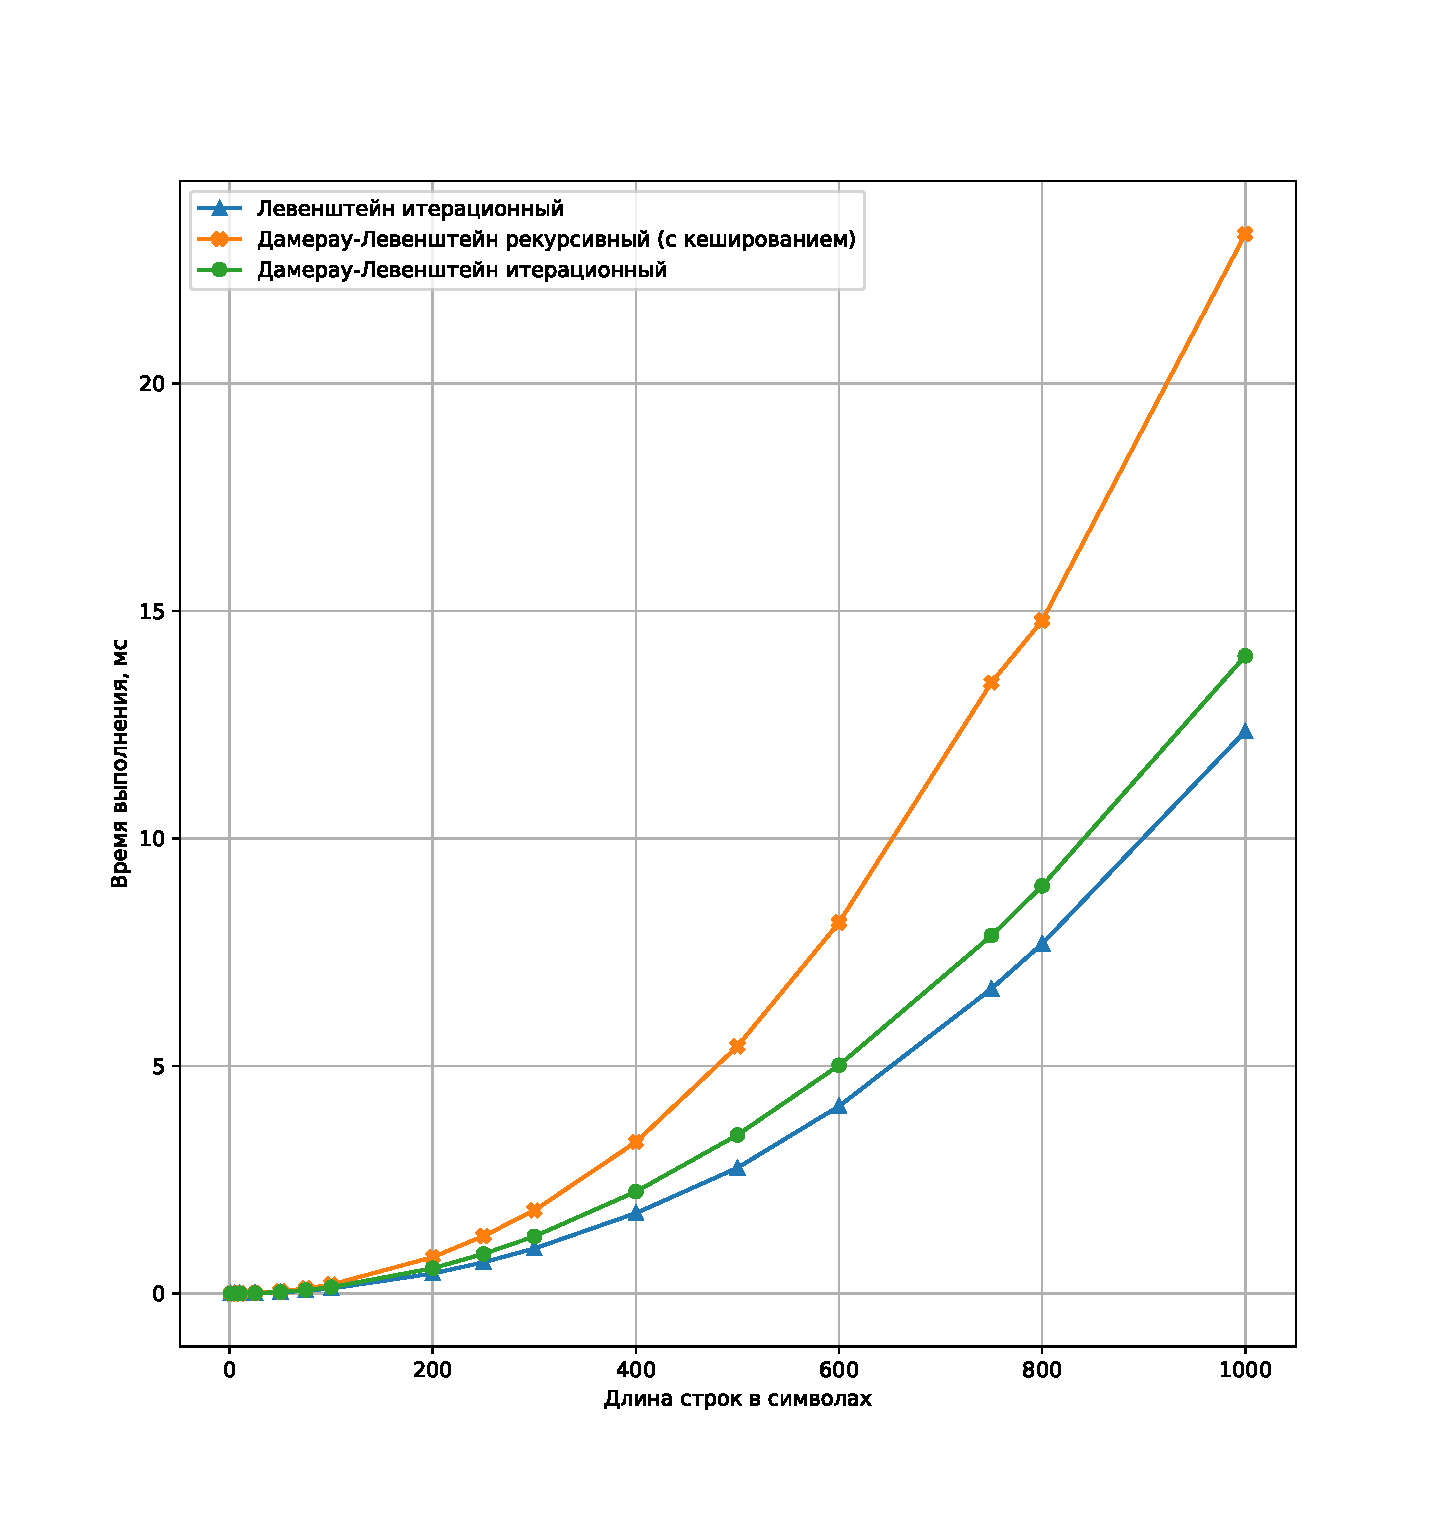
\includegraphics[width=\textwidth]{img/fn_three.pdf}
	\caption{Сравнение итерационных и рекурсивной с кешированием реализаций алгоритмов нахождения расстояний Левенштейна и Дамерау~---~Левенштейна по времени выполнения (среднее время из 100 замеров)}
	\label{fig:fn_three}
\end{figure}

\begin{figure}[H]
	\centering
	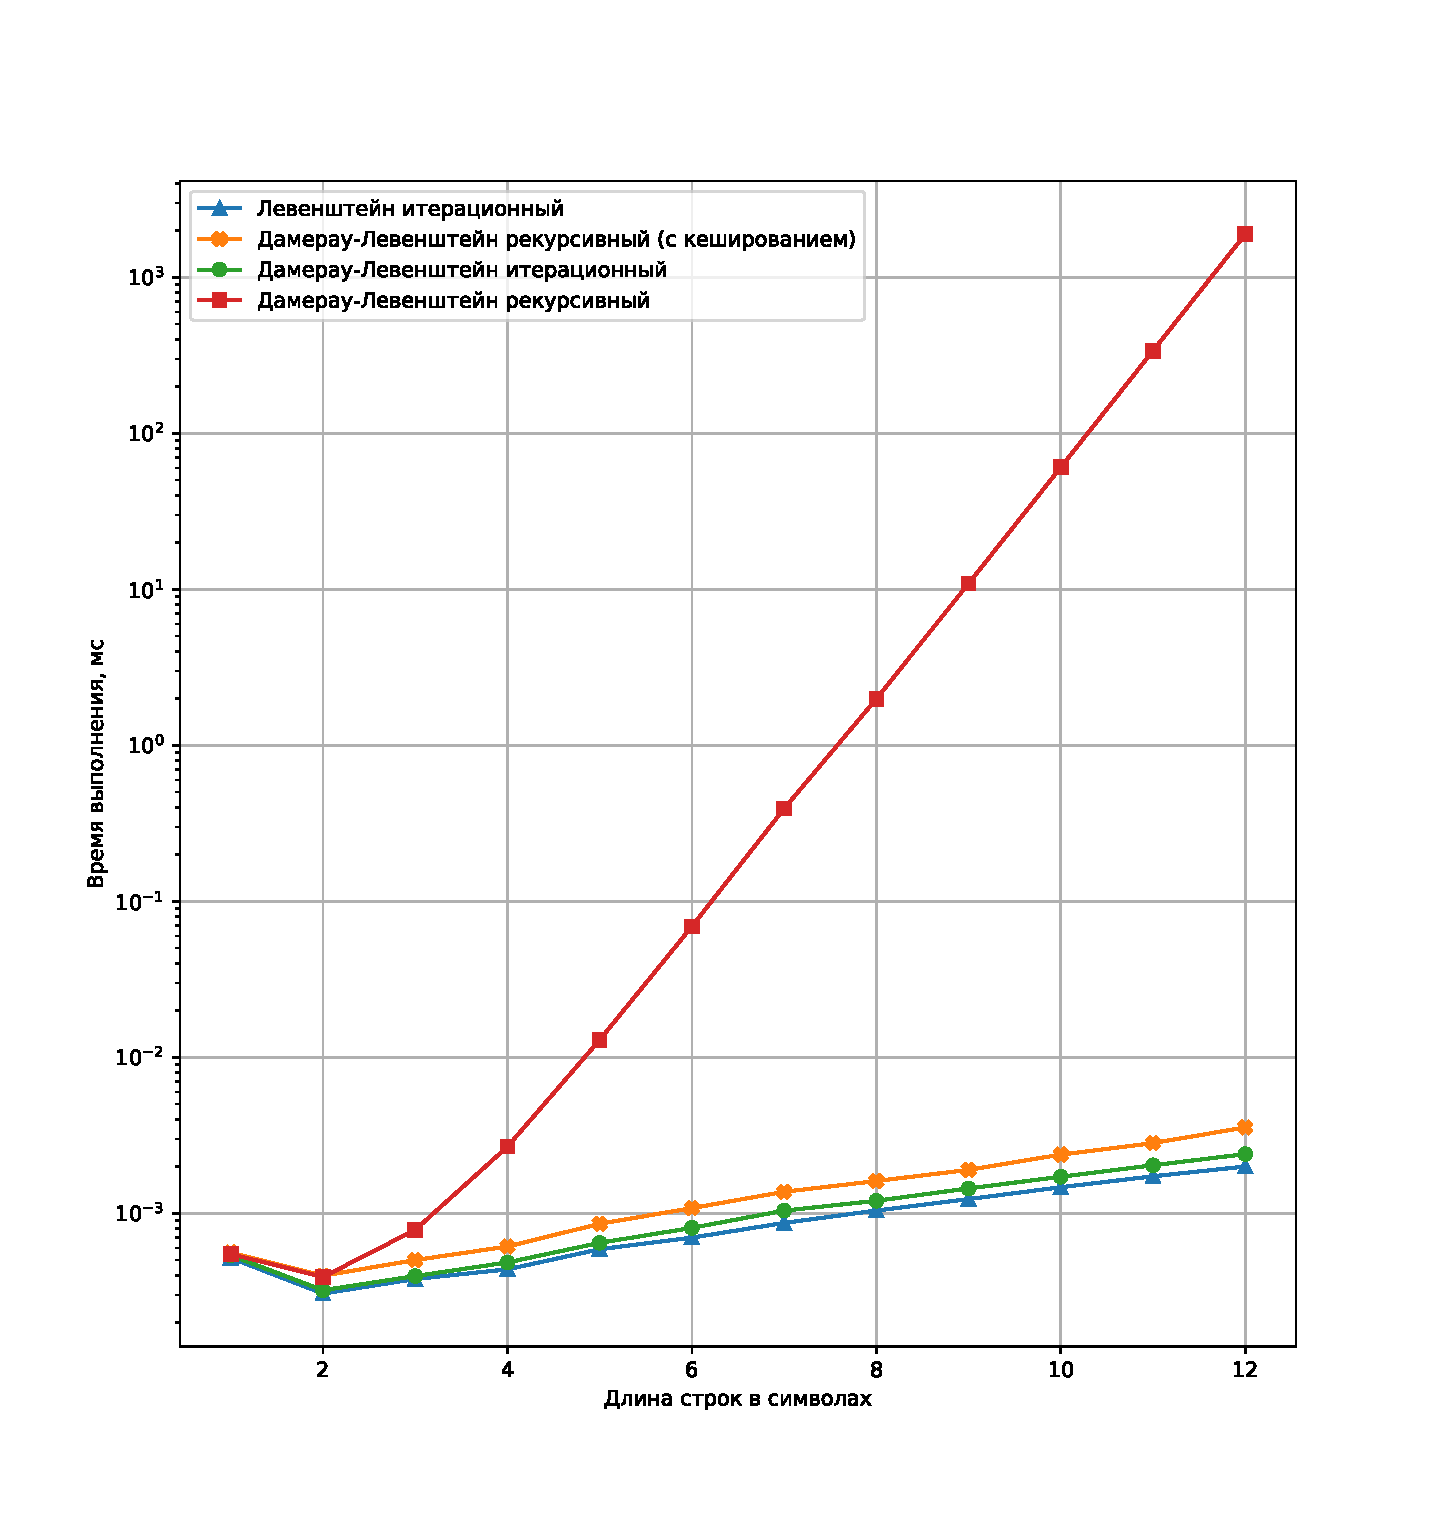
\includegraphics[width=\textwidth]{img/fn_four.pdf}
	\caption{Сравнение всех реализаций алгоритмов по времени выполнения (среднее время из 10 замеров)}
	\label{fig:fn_four}
\end{figure}

\newpage

\subsection{Характеристики по памяти}

\subsection*{Вывод}
